
\documentclass[]{article}

\title{distribucion de frecuencias en el numero de palabras del libro:
 Precepts in Practice; or, Stories Illustrating the Proverbs by A. L. O. E. }

\date{}
\usepackage{braket}
\usepackage{bbold}
\usepackage{amsmath,amsfonts,amssymb,amsthm}
\usepackage[margin=1.0in]{geometry}
\usepackage{graphicx}
\usepackage{chngcntr}
\usepackage{floatrow}
\usepackage{chngcntr}
\usepackage{hyperref}
\usepackage[spanish]{babel}
\counterwithin{figure}{section}
\usepackage[backend=biber]{biblatex}
\addbibresource{ref.bib}
\begin{document}
	\maketitle
	\begin{center}


\centerline{\textbf{TAREA 3} } 
\textbf{ }

\centerline{Alumno: } 
\centerline{Joaquín Arturo Velarde Moreno}


	\end{center}
	

\section{Introducción}
En el presente trabajo se hizo el análisis de la frecuencia en el uso de una selección de palabras contenidas en un texto literario con el objeto de calcular las probabilidades de que aparezcan determinadas palabras con cierto número de letras.

El libro que usamos es el de Precepts in Practice; or, Stories Illustrating the Proverbs del autor A. L. O. E.  \cite{proverbs} 
Este libro se encuentra en la biblioteca digital de Gutenberg  \cite{guten},  el cual es el repositorio de más de 63,127 títulos en formato ebook.

Esta obra que revisamos está escrita en inglés y se conforma por un conjunto de relatos cuyas ilustraciones tienen el objetivo de complementar visualmente cada proverbio y, de acuerdo con este género literario, cada historia conlleva una enseñanza de la que podemos aprender en nuestra vida cotidiana, según las diferentes situaciones y asuntos de que se trate.



\section{Metodología}
Para cumplir con nuestro objetivo, primeramente, procedimos a descargar el texto con el programa “R- 4.0.2” \cite{rproject} , dado que la biblioteca Gutenberg \cite{guten} permite tal descarga libremente.
Como siguiente paso, se removió todo carácter especial no alfa numérico, es decir, los símbolos tipográficos (guiones, cursivas, negritas, etc.) para limpiar el texto.
Debido a que la frecuencia de datos era dominada principalmente por artículos, pronombres personales, conjunciones y números, se hizo una hoja de datos en Microsoft Excel \cite{excel} con este tipo de palabras. Posteriormente, se le ordenó al programa limpiar el texto de dicho contenido.
Con el resto del léxico, se procedió a calcular la frecuencia de las palabras restantes con el programa R para ver las probabilidades de distribución cuantitativa.
Finalmente, se llevó a cabo el análisis para realizar los histogramas utilizando las siguientes cuatro funciones de distribución de probabilidad.

\begin{enumerate}
	\item Distribución geométrica
	\item Distribución hypergeométrica
	\item Distribución binomial negativa
	\item Distribución regular
\end{enumerate}


\subsection{Distribución geométrica}
Con este modelo pudimos observar la probabilidad de obtener palabras con menos de tres letras. 
\autoref{fig:Geometria}

\begin{figure}[b]
    \centering
    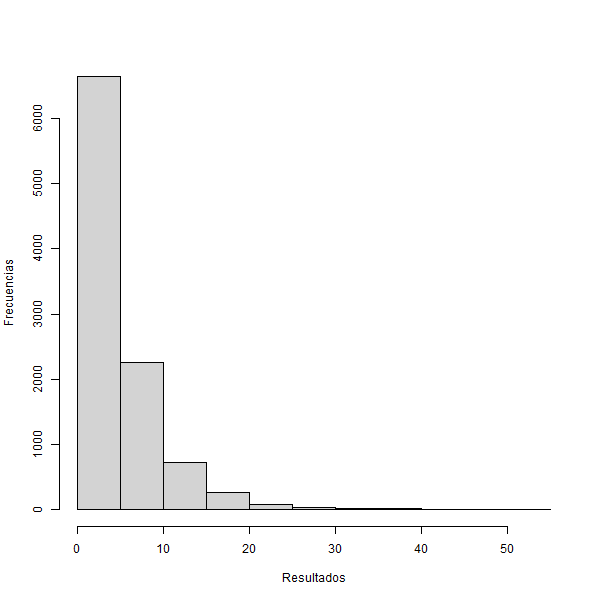
\includegraphics[width=.5\linewidth]{Geometrica.png}    \caption{Probabilidad de que aparezca una palabra con  menos de 3 letras.}
    \label{fig:Geometria}
\end{figure}

\begin{figure}[b]
    \centering
    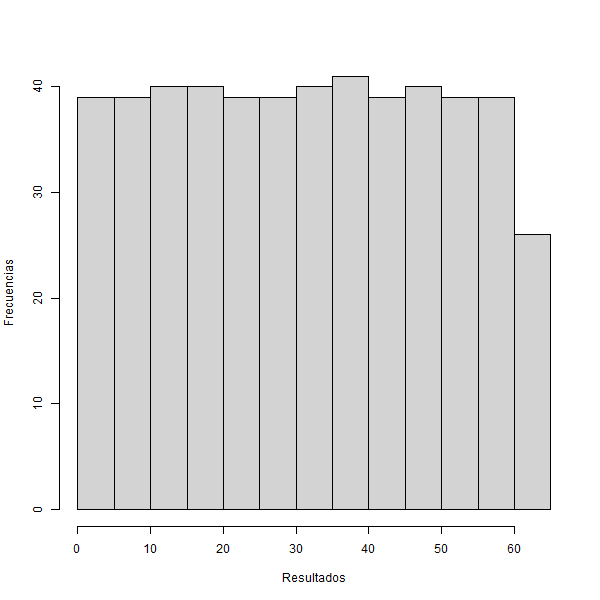
\includegraphics[width=.5\linewidth]{HyperGeometrica.png}    \caption{Probabilidad de que aparezcan 5 palabras con mas de 2 caracteres.}
    \label{fig:HyperGeometrica}
\end{figure}

\subsection{Distribución hypergeométrica}
Con esta distribución, que es primordial en el análisis de muestras pequeñas, se obtiene la probabilidad de que aparezcan cinco palabras que sean mayores de dos caracteres en una muestra de 100 palabras. \autoref{fig:HyperGeometrica}

\subsection{Distribución binomial negativa}
Con esta distribución se repite un experimento hasta juntar un número de casos requeridos de éxito. En nuestro trabajo, con este modelo se obtuvo la probabilidad de 15 palabras conformadas por más de 6 caracteres.\autoref{fig:Negativo}
\subsection{Distribución regular}
Con este modelo se obtiene los resultados de un número determinado de experimentos. En nuestro análisis con la aplicación de dicho modelo se obtuvieron las probabilidades de sacar palabras con más de 7 caracteres. \autoref{fig:Regular}

\begin{figure}[b]
    \centering
    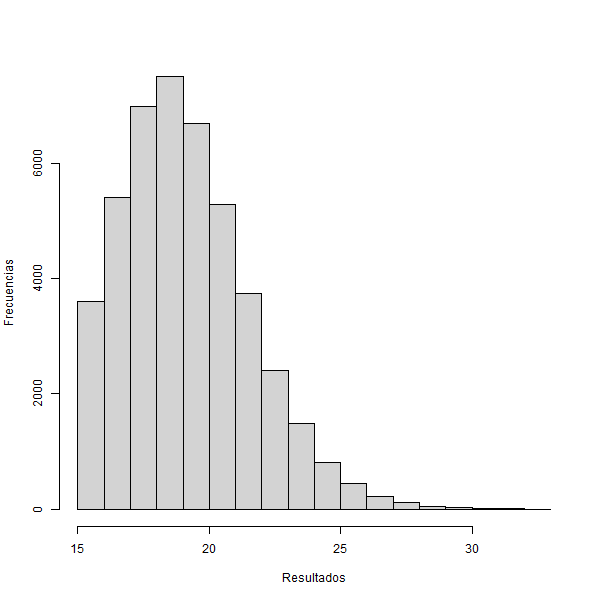
\includegraphics[width=.5\linewidth]{Negativo.png}    \caption{Casos de éxito en donde una palabra es mayor que 6 caracteres.}
    \label{fig:Negativo}
\end{figure}
\begin{figure}[b]
    \centering
    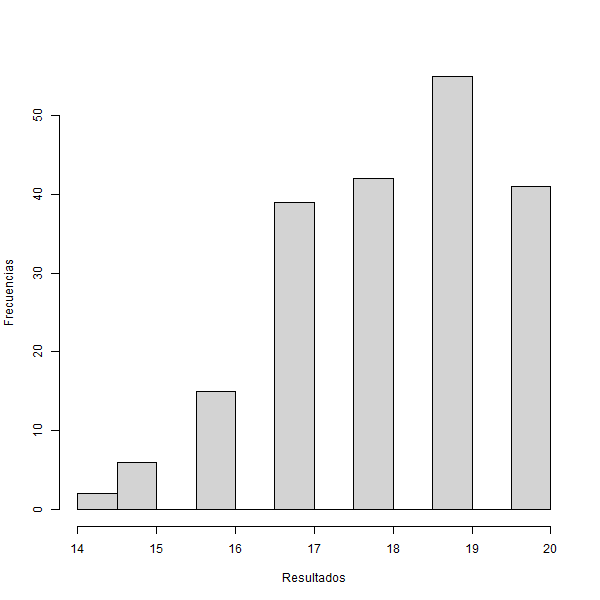
\includegraphics[width=.5\linewidth]{Regular.png}    \caption{Probabilidad de sacar palabras con mas de 7 caracteres.}
    \label{fig:Regular}
\end{figure}


\printbibliography[title={Referencias}]
\end{document}
